%!TEX root = ../report.tex

\begin{document}
    \chapter{Android Deployment}
	\label{chap:androiddeploy}
	
	The Android deployment section explains the procedures for integrating the trained and evaluated semantic segmentation model on an embedded device. The original model was trained and evaluated on a highly computational-powered device, but generally, the embedded device is a low computational device with less energy consumption. In this case, the embedded device used to deploy the segmentation model is an Android One Plus 7 mobile phone with 8 GB of RAM and a Snapdragon 855 processor. Before deploying the model on an Android device, the heavily trained model needs to be optimized to be compatible with the device.    
	
    \section{Framework}
	
	The process of handling a single input image or a sequence is illustrated in Figure \ref{fig:android_pipeline}. The pipeline starts by loading an optimized model and a single image from the media storage in evaluation mode. The image is then passed through the model for prediction. In the final step, the segmented image from the python script is returned to the main Kotlin routine to be displayed. The model is deployed on an Android device with 6 GB of RAM running Android 11. The main routine script is written in Kotlin and integrates with the python script to process the data. The Android device used to deploy the deep learning model is specified in Table \ref{table:android_spec}. The trained model was optimized using the PyTorch \href{https://pytorch.org/docs/stable/mobile_optimizer.html}{\color{teal}mobile optimizer} with evaluation mode modules. The tested Android device takes 13 seconds to read, segment, and display a single input image.
	
	\begin{figure}
		\centering
		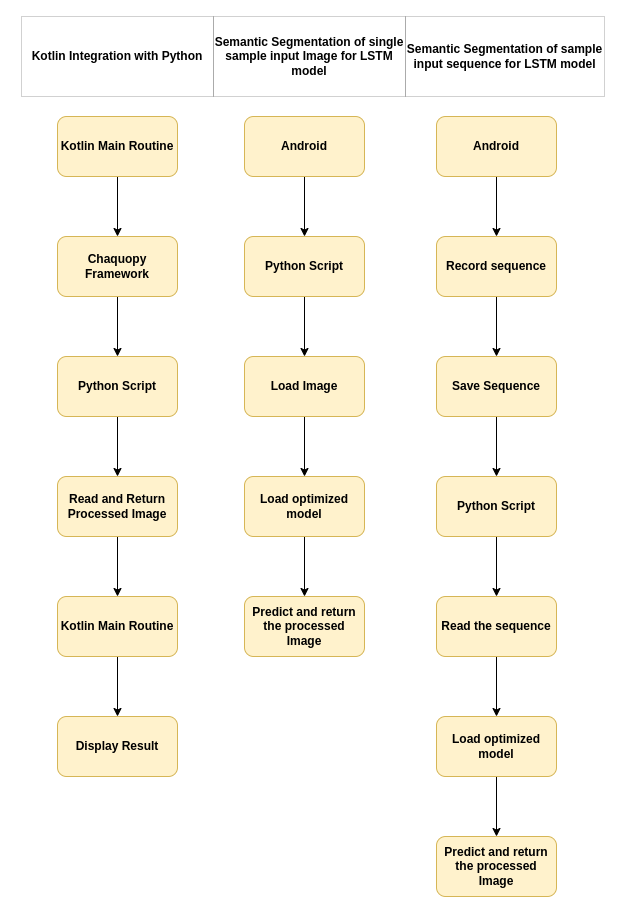
\includegraphics[width=13cm]{images/android_deployment.png}
		\caption{Kotlin integration with python and sequence of steps from loading the image to display of predicted semantic map.}
		\label{fig:android_pipeline}
	\end{figure}
	
	\begin{table}
	\begin{center}
		\begin{tabular}{ | l | p{3cm} |}
			\hline
			
			Device & Oneplus 7 \\ \hline
			Android version & Oxygen OS 11.0.9.1.GM57AA \\ \hline
			Processor & Snapdragon 855 \\ \hline
			RAM & 6 GB 
			\\ \hline
			Model & GM1901 \\ \hline
			\hline
		\end{tabular}
		\caption{Specification of the android device}
		\label{table:android_spec}
	\end{center}
	\end{table}

    \section{Display of results}
	
	The Android application is developed in Kotlin programming language. The layout of the application is shown in Figure \ref{fig:android_result}. The layout consists of six main parts: Heading, Start segmenting the input data, Test Image, Select, Live, and Results display. The Heading is the name of the application, Test Image is the image to be segmented, and any sample image can be selected for segmentation. The Select option allows you to choose images from the media folders and transfer them for processing. The Live option enables live video segmentation and display in real time. Once the target image has been selected, the Start segmenting the input data button initiates the processing of the input data and displays the result on the Android screen. A full description can be found in the image \ref{fig:android_result}. 
	
	\begin{figure}
		\centering
		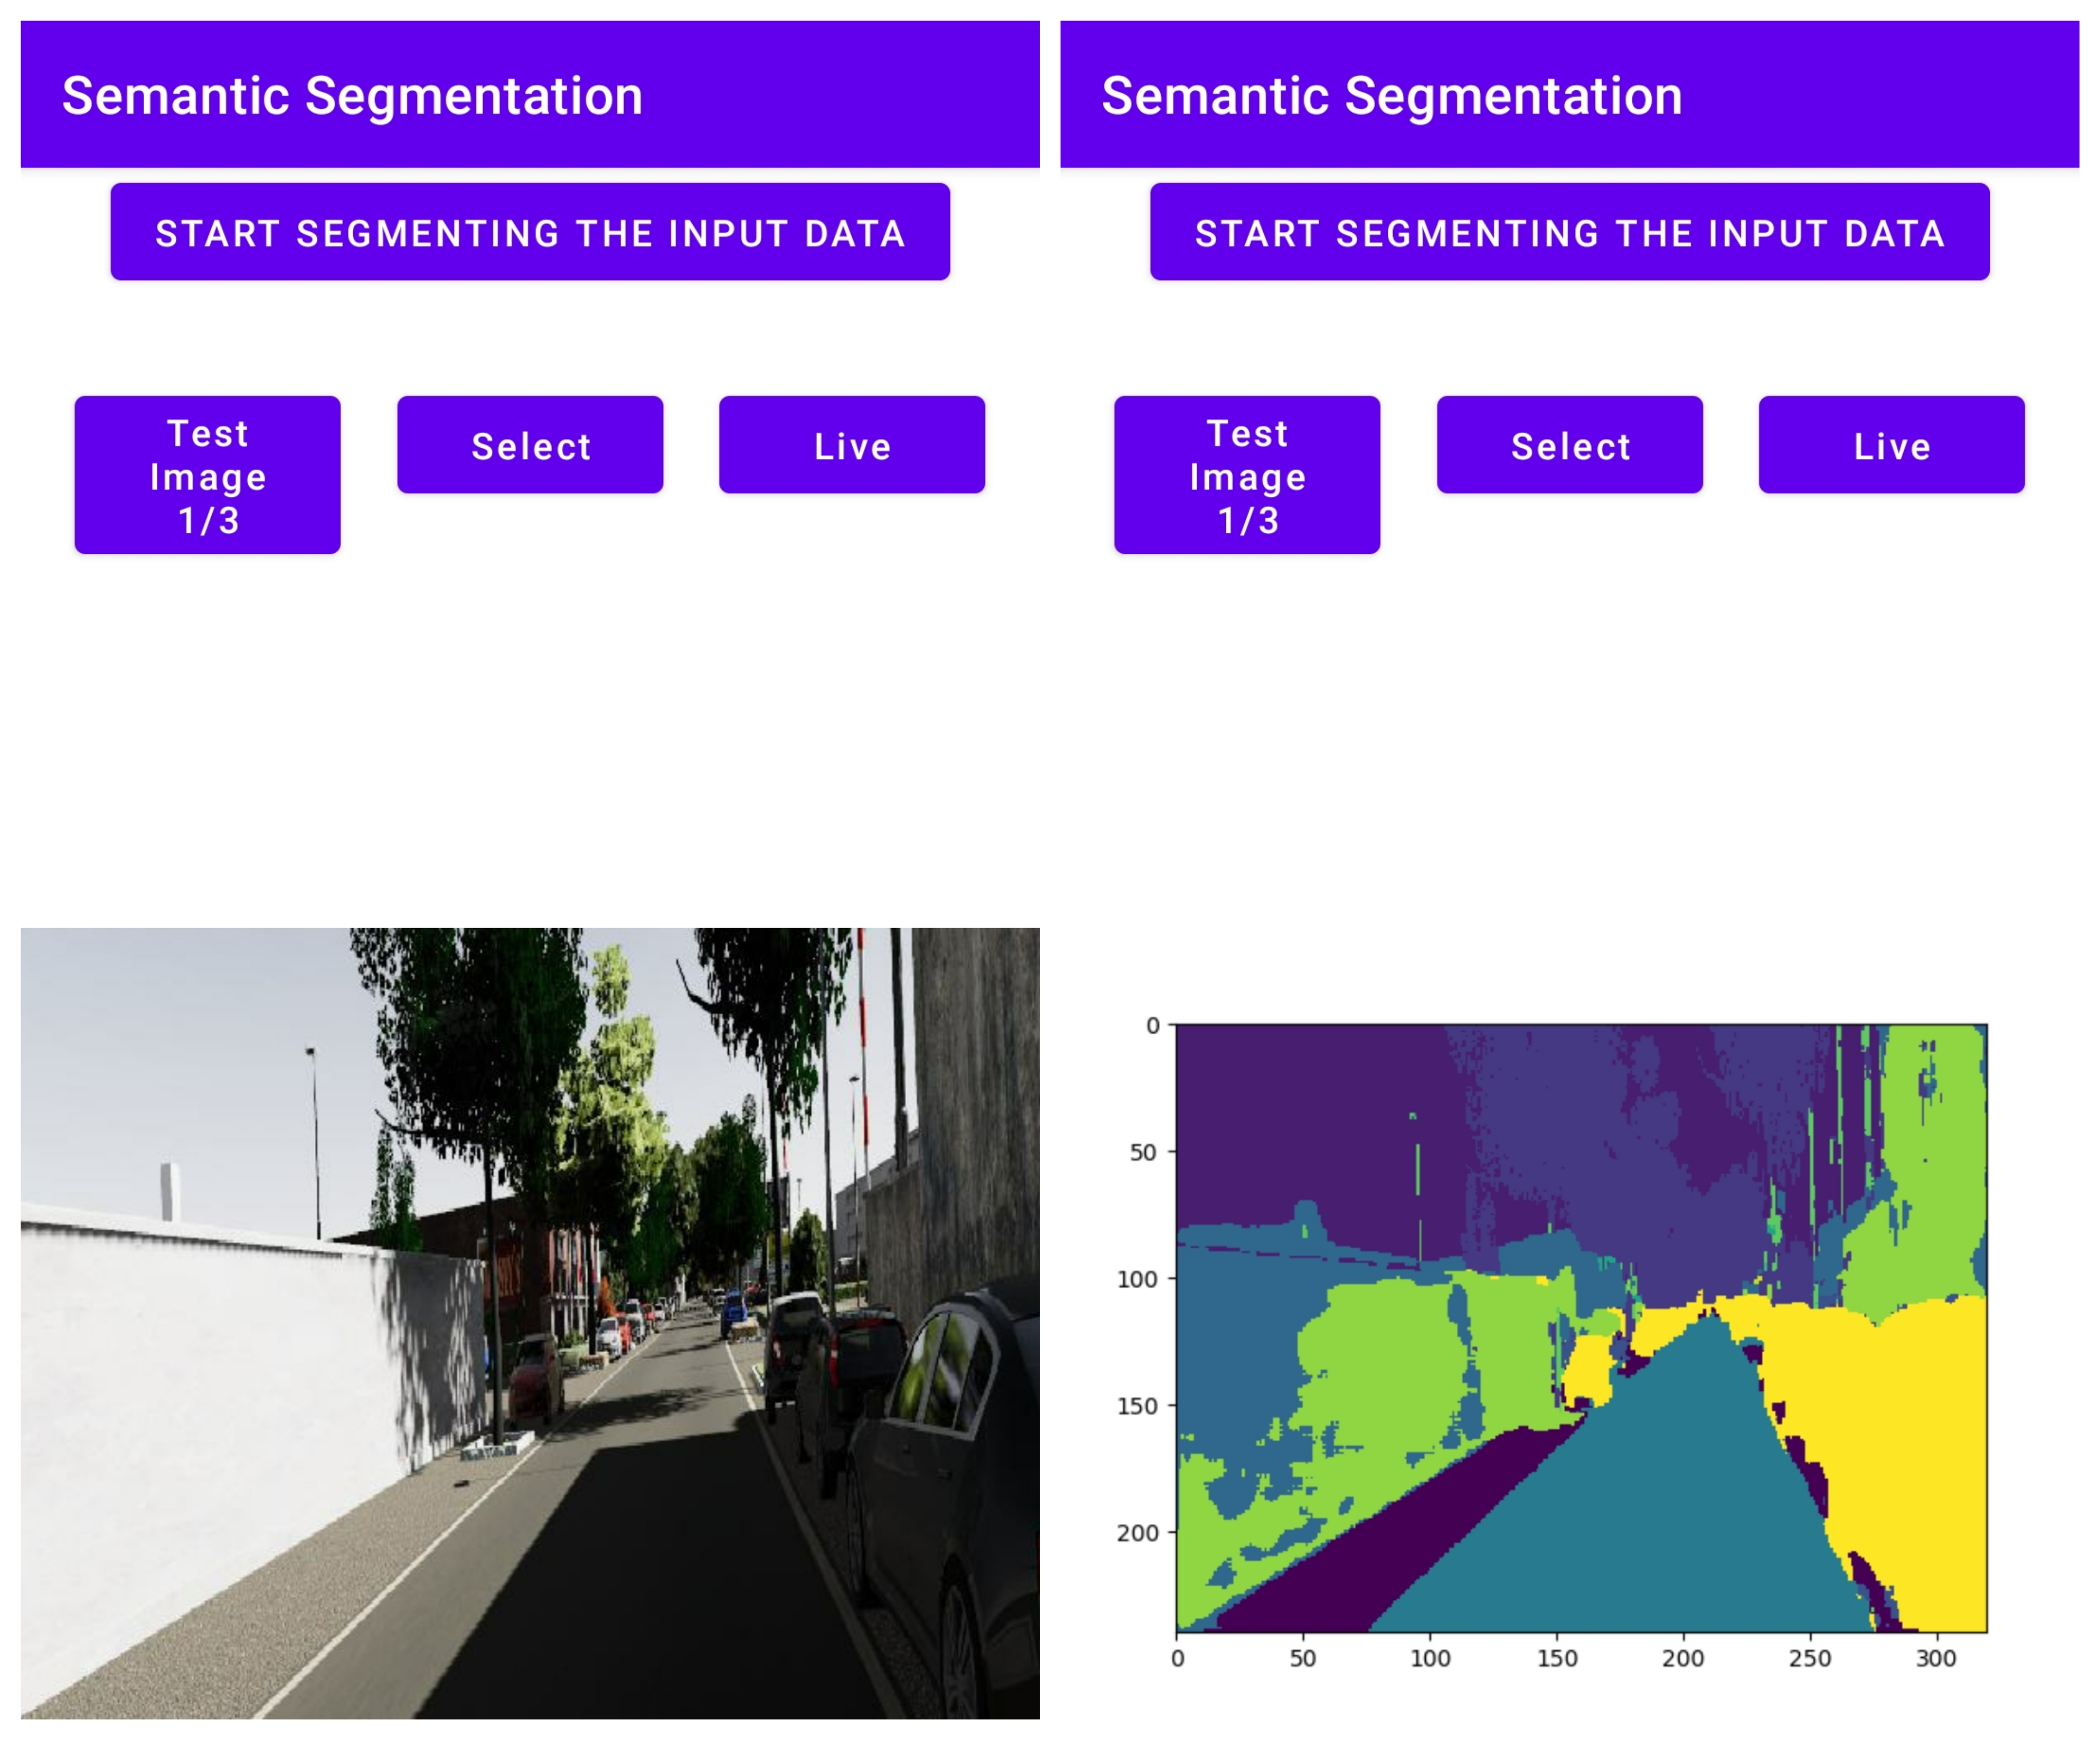
\includegraphics[width=13cm]{images/android_ss.jpg}
		\caption{Display of loading the image and predicted semantic map}
		\label{fig:android_result}
	\end{figure}
    
    \newpage
    \section{Runtime}
	
	The android device is subjected with a sample input and the response time is tabulated in the table \ref{table:response_of_android}. The sample is a single frame from the video sequence data. The image goes through multiple stages starting from reading the image to processing and display of the results. 
	
	\begin{table}[h]
		\begin{center}
			\begin{tabular}{ | l | p{3cm} |}
				\hline
				
				Android version & Oxygen OS 11.0.9.1.GM57AA \\ \hline
				Image Loading time & 2 seconds \\ \hline
				Image processing & 9 seconds \\ \hline
				Display of result & 2 seconds \\ \hline
				Total & 13 seconds \\ \hline
				\hline
			\end{tabular}
			\caption{Runtime detail for processing of single image}
			\label{table:response_of_android}
		\end{center}
	\end{table}    
    
\end{document}
